\documentclass[12pt,english]{article}
\usepackage[a4paper,left=3cm,right=2cm,top=2.5cm,bottom=2.5cm]{geometry}
\usepackage[utf8]{inputenc}
\usepackage[english]{babel}
\usepackage{graphicx}
\usepackage{pifont}
\usepackage{color}
\usepackage{xcolor}
\usepackage{colortbl}
\usepackage{amsthm,thmtools}
\usepackage{multirow}
\usepackage{amsmath}
\usepackage{subcaption}
\usepackage{adjustbox}
\usepackage{url}
\usepackage{svg}
\usepackage{multirow}
\usepackage[hidelinks]{hyperref}
\usepackage{caption}
\usepackage{apacite}
\usepackage{amsthm}
\usepackage{multicol}
\usepackage{float}
\usepackage{amsfonts}
\usepackage[usestackEOL]{stackengine}
\usepackage{titling}
\usepackage{soul}
\usepackage{pgfplots}
\usepackage[nottoc]{tocbibind}
\usepackage{listings}
\usepackage{array}
\usepackage[framemethod=tikz]{mdframed}
\usepackage{footnote}
\makesavenoteenv{tabular}
\makesavenoteenv{table}
\newcommand{\greentick}{\textcolor{green}{\ding{52}}}
\newcommand{\redcross}{\textcolor{red}{\ding{55}}}
\graphicspath{ {./img/}}
\makeatletter
\def\input@path{{input/}}
\makeatother
\selectlanguage{english}
%\usepackage{fancyhdr}
%\pagestyle{fancy}
\usepackage[
    type={CC},
    modifier={by-nc-sa},
    version={4.0},
]{doclicense}


\lstset{
  breaklines=true,
  postbreak=\mbox{\textcolor{red}{$\hookrightarrow$}\space},
}
\lstdefinelanguage{docker-compose}{
  keywords={image, environment, ports, container_name, ports, volumes, links},
  keywordstyle=\color{blue}\bfseries,
  identifierstyle=\color{black},
  sensitive=false,
  comment=[l]{\#},
  commentstyle=\color{purple}\ttfamily,
  stringstyle=\color{red}\ttfamily,
  morestring=[b]',
  morestring=[b]"
}

\makeindex

\definecolor{light-gray}{gray}{0.95}
\lstset{columns=fullflexible,basicstyle=\ttfamily}
\surroundwithmdframed[
  hidealllines=true,
  backgroundcolor=light-gray,
  innerleftmargin=0pt,
  innertopmargin=0pt,
  innerbottommargin=0pt]{lstlisting}

\pgfplotsset{width=8cm,compat=1.9, xlabel={Year},
  ylabel={Number of documents}, xtick distance={2},
  ytick distance={2}, ymajorgrids=true,grid style=dashed,
  /pgf/number format/.cd,use comma,1000 sep={}}


\begin{document}

\begin{titlepage}

 \newlength{\centeroffset}
 \setlength{\centeroffset}{-0.5\oddsidemargin}
 \addtolength{\centeroffset}{0.5\evensidemargin}
 \thispagestyle{empty}

 \noindent\hspace*{\centeroffset}
 \begin{minipage}{\textwidth}

  \centering
  
\includegraphics[width=0.9\textwidth]{logo_ugr.jpg}\\[1.4cm]

  \textsc{ \Large Bachelor Final Project\\[0.2cm]}
  \textsc{Computer Engineering}\\[1cm]

  {\Huge\bfseries HOW-R-U?\\}
  \noindent\rule[-1ex]{\textwidth}{3pt}\\[3.5ex]
  {\large\bfseries Analising chatbot messages to automatically infer human behaviour}
 \end{minipage}

 \vspace{1cm}
 \noindent\hspace*{\centeroffset}
 \begin{minipage}{\textwidth}
  \centering

  \textbf{Author}\\ {Carlos Sánchez Páez}\\[2.5ex]
  \textbf{Supervisor}\\
  {Oresti Baños Legrán}\\[3ex]
  
\includegraphics[width=0.4\textwidth]{etsiit_logo.png}\\[0.1cm]
  \vspace{2.5ex}
  
\includegraphics[width=0.15\textwidth]{atc.jpg}\\[0.1cm]
  \vspace{1cm}
  \textsc{Escuela Técnica Superior de Ingenierías Informática y de Telecomunicación}\\
  \vspace{1cm}
  \textsc{Granada, academic year 2019-2020}
 \end{minipage}
\end{titlepage}


\cleardoublepage
\thispagestyle{empty}

\begin{center}
{\large\bfseries  HOW-R-U?: Suite of e-coaches aimed to analyse human behaviour}\\
\end{center}
\begin{center}
Carlos Sánchez Páez\\
\end{center}

%\vspace{0.7cm}
\noindent{\textbf{Palabras clave}: chatbot, telegram, salud, médico, asistente, coach, suite}\\

\vspace{0.7cm}
\noindent{\textbf{Resumen}}\\

Hoy en día los trastornos mentales siguen siendo difíciles de tratar y diagnosticar. Además, debido al estigma que conllevan, algunos de los posibles pacientes no se sienten cómodos acudiendo a un profesional de la psicología. El objetivo de este proyecto es desarrollar una suite de e-coaches en forma de chatbots, específicamente, un chatbot de salud mental que ayude al diagnóstico prematuro de enfermedades mentales como la ansiedad y la depresión. Esta suite será modular, de forma que cada especialista pueda tener un agente conversacional asociado (psicólogo, nutricionista, etc.). Además, se le incorporará funcionalidad para que sea útil no solo para doctores, sino para analistas de datos, que contarán con la información recopilada de todos los pacientes.\\

Se plantea como trabajo futuro el uso de este sistema en un entorno en el que el asistente iniciará una conversación regularmente con el paciente y le hará una serie de preguntas definidas por su doctor. Tras ello, el especialista podrá acceder a una interfaz web en la que consultará y analizará las distintas respuestas proporcionadas por el paciente.
\cleardoublepage


\thispagestyle{empty}


\begin{center}
{\large\bfseries HOW-R-U?: Suite of e-coaches aimed to analyse human behaviour}\\
\end{center}
\begin{center}
Carlos Sánchez Páez\\
\end{center}

%\vspace{0.7cm}
\noindent{\textbf{Keywords}: chatbot, telegram, health, doctor, assistant, coach, suite}\\

\vspace{0.7cm}
\noindent{\textbf{Abstract}}\\

Nowadays mental ilnesses are still difficult to be treated and diagnosed. Moreover, they are associated to a stigma, so some possible patients do not feel comfortable when requesting profesional help. The aim of this project is to develop an e-coaches suite as chatbots, specifically a mental health chatbot
that would help to the premature diagnostic of mental illnesses such as anxiety and depression. This suite will be modular so that every specialist can have an associated conversational agent (psychologist, nutritionist, etc.). Moreover, it will also support data analysts, special doctors that will be able to consult all the information from all the patients.\\

It is proposed the use of this system in an environment where the assistant will regulary start a conversation with the patients, making them questions defined by their doctors. After that, the specialists will be able to access a web interface where they can consult and analyze the answers given by patients.

\newpage

\section*{}
\thispagestyle{empty}

\noindent\rule[-1ex]{\textwidth}{2pt}\\[4.5ex]

Yo, \textbf{Carlos Sánchez Páez}, alumno de la titulación Graduado en Ingeniería Informática de la \textbf{Escuela Técnica Superior
de Ingenierías Informática y de Telecomunicación de la Universidad de Granada}, con DNI 25613096C
, autorizo la
ubicación de la siguiente copia de mi Trabajo Fin de Grado en la biblioteca del centro para que pueda ser
consultada por las personas que lo deseen.

\vspace{6cm}

\begin{center}
  Fdo: Carlos Sánchez Páez

\end{center}

\vspace{2cm}

\begin{flushright}
Granada a 01 de julio de 2020
\end{flushright}

\newpage

\section*{}
\thispagestyle{empty}

\noindent\rule[-1ex]{\textwidth}{2pt}\\[4.5ex]

D. \textbf{Oresti Baños Legrán}, Profesor del Departamento Arquitectura de Computadores de la Universidad de Granada.



\vspace{0.5cm}

\textbf{Informa:}

\vspace{0.5cm}

Que el presente trabajo, titulado \textit{\textbf{HOW-R-U?: Suite of e-coaches aimed to analyse human behaviour}},
ha sido realizado bajo su supervisión por \textbf{Carlos Sánchez Páez}, y autorizo la defensa de dicho trabajo ante el tribunal
que corresponda.

\vspace{0.5cm}

Y para que conste, expide y firma el presente informe en Granada a 01 de julio de 2020

\vspace{1cm}

\textbf{El supervisor:}

\vspace{5cm}
\begin{center}
\textbf{Oresti Baños Legrán}

\end{center}


\newpage

\section*{Agradecimientos}
\thispagestyle{empty}

\vspace{1cm}
\begin{flushleft}
A mi familia, porque sin ellos nunca habría llegado tan lejos.

A Cristina, por su apoyo incondicional en todo momento.

A Casandra, por haber estado conmigo desde el principio.

A Oresti, por haberme apoyado en momentos difíciles y ser una gran fuente de motivación y conocimiento.

Al los buenos profesores que he encontrado durante mi carrera académica, por haber sabido enseñar y motivar.

Al mis amigos y amigas, por haberme ayudado siempre que lo he necesitado.
\end{flushleft}

\thispagestyle{empty}
\newpage
\tableofcontents{}
\newpage
%\listoffigures
%\thispagestyle{empty}
%\newpage
%\rhead{}
%\lhead{}
%\renewcommand{\headrulewidth}{0pt}
%\renewcommand{\footrulewidth}{0pt}
\section{Introduction}
\subsection{Context}

Mental disorders are very common in our society. According to \cite{Bandelow2015}, almost 34\% of the population suffer from anxiety at least once in their lives. They are difficult to be diagnosed and properly treated. Most intervention programs do not last as much as they should and doctors have a very high workload, so patients need to wait for a long time before being advised by a doctor. In addition, although having a mental disease is very common, it is still a taboo subject whose stigma makes them even more difficult to be diagnosed and treated, as \cite{Davies2000} states.\\

In addition, people do not go to the doctor every time something happens, so there is not a continuous traceability of patients' health status. This causes a lot of relevant data not to be retrieved. This data could be suitable to perform more specific and personal medical analysis. Having a coach that regularly interacts with the person with a mental disorder as well as extracts data from his or her responses would take advantage of this information.


\subsection{Motivation}

Nowadays, technology is becoming increasingly integrated in our lives. Specifically, smartphones have became a daily basis used tool. People read the news, check the weather, chat with their relatives and friends, etc. using smartphones. Modern chat applications (such as \cite{Telegram}) allow people to create bots that can interact with them like if there was a person on the other side. These chatbots are increasingly becoming popular amongst people because they cover many functionalities, from tracking shipments to playing games and reminding stuff. Telegram bots do not require another app to be installed in the client's phone, so the client can save storage space.\\

As we previously discussed, mental disorders are taboo, so having a bot you could talk with about how was your day, feelings, etc. could lead to an easier way of diagnosing them because chat conversations are seen as ''natural'' by society. The conversational agent will ask the patient a batch of questions (previously defined by his/her doctor) and show the data to the specialist so that the diagnosis can be more precise.

\newpage

\subsection{Objectives}

\begin{itemize}
  \item \textbf{Main goal}: to develop a conversational agent as a sensor which will be able to interact with a person with a mental disorder in a natural way and ask questions defined by specialists.
  \item \textbf{Secondary goals}:
    \begin{itemize}
      \item To design a graphical web interface where doctors can consult their patient's responses.
      \item To design a flexible and scalable architecture to add functionality to the conversational agent.
      \item To design an architecture based on containers to host the different system modules.
      \item To implement a system that covers the previous goals.
      \item To test a beta version of the assistant in real people and analyse the retrieved data as well as target audience's feelings about it.
    \end{itemize}
\end{itemize}

\subsection{Structure}

The first chapter of this project offers an introduction to the context in which the main goal is intended to be developed as well as an analysis of related papers. This section is divided into four main categories (health application domains, conversational agents types, communication format and architecture) and a research about the popularity of chatbots.\\

The second one (\textbf{Methodology}) contains the proper requisites design, architecture, programming language and frameworks that are intended to be used in the system development, as well as its the most important modules and some code snippets to illustrate its functionality.\\

The third one, \textbf{Evaluation}, shows the results of the application testing amongst real people and the obtained results in an objective way.\\

The fourth chapter, \textbf{Discussion}, analyses the results obtained in the third chapter.\\

Finally, the last one, \textbf{Conclussions} analyses the initial objectives of the project and if they were achieved or not.



\newpage

\section{State of the art}

\subsection{Number of publications related to chatbots}

Several queries were performed on \textit{scopus.com} to check the number of articles per year related to chatbots and their applications in health. The obtained results were the following ones:

\begin{figure}[H]
  \begin{subfigure}[t]{0.3\textwidth}
    \centering
    \begin{tikzpicture}
      \begin{axis}[title=\shortstack{chatbot OR "conversational agent"}, ytick distance={100}]
        \addplot table {data/chatbot_or_ca_query_results.dat};
      \end{axis}
    \end{tikzpicture}
  \end{subfigure}
  \hspace{3cm}
  \begin{subfigure}[t]{0.3\textwidth}
    \centering
    \begin{tikzpicture}
      \begin{axis}[title=\footnotesize{\shortstack{(chatbot OR "conversational agent")\\AND\\(coach OR counselor OR assistant)}},
                   ytick distance={15}]
        \addplot table {data/chatbot_or_ca_and_coach_or_counselor_or_assistant_query_results.dat};
      \end{axis}
    \end{tikzpicture}
  \end{subfigure}

  \vspace{0.5cm}

  \begin{subfigure}{\linewidth}
    \centering
    \begin{tikzpicture}
      \begin{axis}[title=\footnotesize{\shortstack{(chatbot OR "conversational agent")\\AND\\(coach OR counselor OR assistant)\\AND\\health}}, ytick distance={5}]
        \addplot table {data/chatbot_or_ca_and_coach_or_counselor_or_assistant_and_health_query_results.dat};
      \end{axis}
    \end{tikzpicture}
  \end{subfigure}
  \caption{Search results of different queries performed in \textit{scopus.com}}
\end{figure}

We can observe that, in the last 5 years, all of them show a considerable increasing number of articles and papers related to virtual assistants.


\subsection{Health application domains}

Chatbots can be applied to many health domains. For example, \cite{Alesanco2017185} proposes an agent that provides help to perform dermatological medicament prescriptions. \cite{BennetPraba20193470} takes care about nutrition by proposing a chatbot to motivate patients to maintain weight. Another example of conversational interface oriented to health is \cite{Falala-Sechet2019236}. This paper is about establishing a dialogue with patients to help them go through difficult situations that can affect their psychological status.\\

Chat agents can not only be classified according to the area they area applied to, but also according to the objective public. We can distinguish chatbots to help students learn, such as \cite{Lopez2008194} proposal, that offers a simulation of a real patient that presents several symptoms so that students have to interview it and make a diagnostic as a doctor would do in real life. Other interesting project is \cite{Shorey2019e14658}, that intends to improve communication between patients and hospital workers by making virtual patients simulate clinical scenarios so that undergraduates could practise with real situations instead of standard ones.\\

There are also chatbots aimed to help doctors do their work. For example, \cite{Ni201738} offers an agent that interviews sick people before the doctor does. Mandy elaborates a diagnostic based on several questions about patients symptoms and sends it to the doctor so that he can save that time. As professional treatments do not last as much, complements such as \cite{DAlfonso2017} are used. They offer a long-term treatment after the professional one so that the patient's progress is not lost. \\

Virtual agents can be also aimed to help patients. For example, \cite{Harilal2020349} is a counsellor that helps patients with depression by establishing empathetic conversations with them. \cite{Roca2020954} suggests an agent that offers help to people by reminding the intake of their medication, sending notifications to caregivers, providing summaries, etc.

Health coaches can be really helpful. For example, \cite{Breso2016297} proposes a platform to identify and provide early intervention for symptoms of depression and suicide. Its usability percentage was 75.7\% and its accuracy, 70.9\%. Another example is \cite{Hirano2017}, which offers preventive therapy for mental healthcare. The audience's mental health punctuation significantly improved after using the application. Moreover, the usage rate and the number of suggested actions carried out was high. That indicates that people found the app useful. By last, \cite{Ring2016} suggests an agent that responds to users' affective states during virtual therapy sessions. Facial expressions and voices are measured during the session. 70\% of users affirmed that they felt understood by the agent. 50\% of them stated that the agent evoked emotional responses in them during the interactions.

\newpage
\subsection{Conversational agents types and communication formats}

Virtual assistants can be classified attending to their main goal. Coaches help the user to get what he wants. For example, \cite{HUDLICKA2013160} presents a coach that assists people while trying to meditate by motivating them to do it. The paper's results showed that using the agent was more effective in helping users to establish a regular meditation habit. \cite{Guo2020} offers another coach that asseses users in their workouts to improve their postural hygiene by using wearables as sensors. Conversational agents can also be counselors (they help the user to identify and solve problems). The research carried out by \cite{Drislane2020158} proves that counselors can be really helpful when trying to reduce alcohol and drugs consumption amongst users. \cite{Yasavur2014381} suggests a virtual therapist that gives brief speech interventions (3-5 minutes) aimed to let a person's alcohol consumption up and make him or her be aware of the problem. \\

They can use different methods to communicate with their audience: text, voice or both. If we focus on speech-enabled conversational agents, we can distinguish \cite{Maharjan2019929}, which proposes a smart speaker that regularly asks its audience about their sleep quality, mood and physical activity. By analysing the given responses and their tone, volume and  intonation the agent is able to extract useful information useful for detecting markers of a possible mental ilness. In text-based chatbots, the user's input can be free (the agent will translate it to an ontology to understand it) or limited (a custom keyboard with fixed options will be shown or the agent will ask the user to enter a valid option). Finally, the most popular virtual assistants are multimodal (they both admit text and speech communication).

\begin{figure}[H]
  \centering
  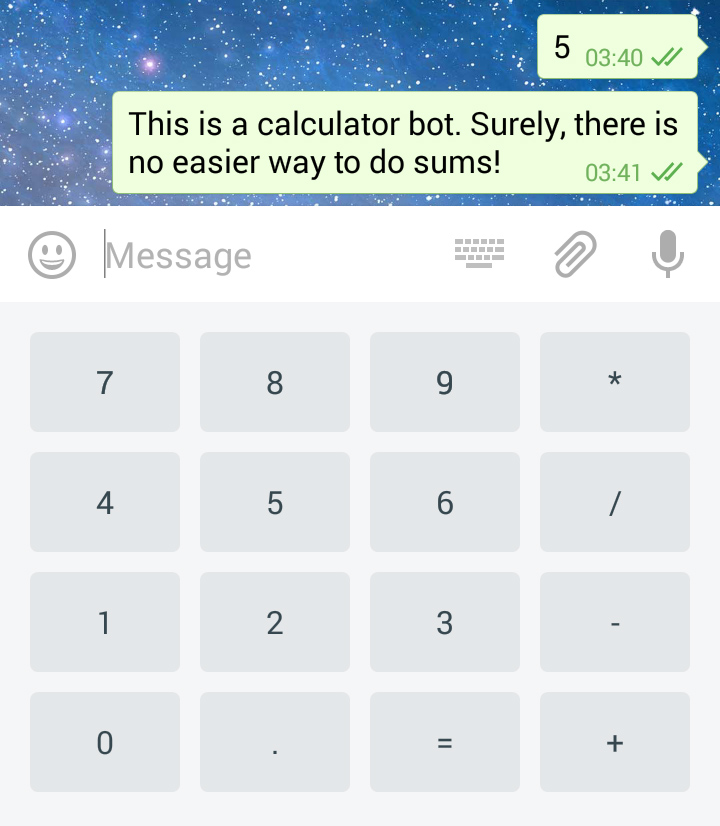
\includegraphics[scale=0.2]{custom_keyboard.jpg}
  \caption{Example of a custom keyboard for a conversational agent}{Reprinted from https://core.telegram.org/bots}
\end{figure}


A review of each of the previous sections can be seen in \cite{Montenegro201956}.
\newpage
\subsection{Technology}

After performing some research, the following table was elaborated:

\begin{table}[h!]
  \centering
  \begin{tabular}{|c|c|c|c|}
    \hline
    \textbf{Platform} & \addstackgap{\textbf{\shortstack{Number of daily \\ active users}}} & \textbf{Free API to implement chatbots}  \\
    \hline
    \cite{FacebookMessenger} & 1.66 billion &  \greentick  \\
    \hline
    \cite{Whatsapp} & 1.5 billion & \redcross \\
    \hline
    \cite{WeChat} & 1.083 billion & \greentick  \\
    \hline
    \cite{Telegram} & 0.2 billion & \greentick \\
    \hline
    \cite{Kik} & 0.015 billion & \greentick \\
    \hline
    \cite{Discord} & 0.014 billion & \greentick \\
    \hline
    \cite{Slack} & 0.012 billion &  \greentick \\
    \hline
    \cite{Viber} & 0.008 billion &  \greentick \\
    \hline
    \cite{Line} & 0.00723 billion & \greentick  \\
    \hline
  \end{tabular}
  \caption{Comparison between different chat applications (2019)}
\end{table}


We can see that Whatsapp, which is the most used messaging app, has no free API to develop conversational agents (the one it has it oriented to business). As opposed, the rest of the widely used chat applications offer an API for programmers to build chatbots in an easy way. \\

A key aspect on social networks is the privacy they ensure. \cite{Kosinski5802} shows that Facbook's likes can be helpful to predict people's sensitive attributes such as age, gender or happiness. \cite{Rastogi17} affirms that Whatsapp's end-to-end encryption methods are not secure enough as metadata can reveal private information. On the other hand, \cite{Sutikno16} states that Telegram provides more privacy protection than other apps. One of its main features is that users can create and customize an username so that they don't have to exchange phone numbers to chat (such as in Whatsapp).


\newpage

\section{Methodology}

\subsection{Design}

\subsubsection{Requirements}
MoSCoW prioritization method \cite{moscow} will be used to classify the requirements of this project. MoSCoW is an acronym for ''\textbf{M}ust have, \textbf{S}hould have, \textbf{C}ould have and \textbf{W}on't have'', categories in which requirements are divided.
\begin{itemize}
  \item \emph{Must have} requirements. They are critical to the success of the project.
    \begin{itemize}
      \item The conversational agent must ask questions defined by doctors to the patients.
      \item The conversational agent must have a custom keyboard with the possible question answers.
      \item The application must allow doctors and patients enrollment.
      \item The system must provide an interface to show the retrieved data.
      \item The system must support modularity.
    \end{itemize}
  \item \emph{Should have} requirements. These are important requirements, but not necessary for  the system release.
    \begin{itemize}
      \item The system should be under a CC BY-NC-SA 4.0 \cite{CC} license.
      \item The application should allow the doctors to add, modify and delete questions and their respective answers.
      \item The application should generate plots to show the collected data to the doctors.
      \item The conversational agent should support audio and text messages.
      \item The conversational agent should be able to ask questions following a configurable schedule.
    \end{itemize}
  \item \emph{Could have} requirements. Desirable requirements that could improve user's experience or satisfaction. Will be included if there is time at the end of the development.
    \begin{itemize}
      \item The system could be translated to other languages.
      \item The application could support password recovery functionality for doctors.
      \item The application could support two factor authentication for doctors.
      \item The conversational agent could support videomessages.
      \item The conversational agent could support groups.
    \end{itemize}
  \item \emph{Won't have} requirements. They are inappropiate or the least important ones, so they are not included in the project.
    \begin{itemize}
      \item The application won't be cross-platform.
      \item The system won't share the retrieved data with third parties.
    \end{itemize}
\end{itemize}
\newpage
\subsubsection{Architecture}
The proposed system will implement the following architecture:
\begin{figure}[H]
  \centering
  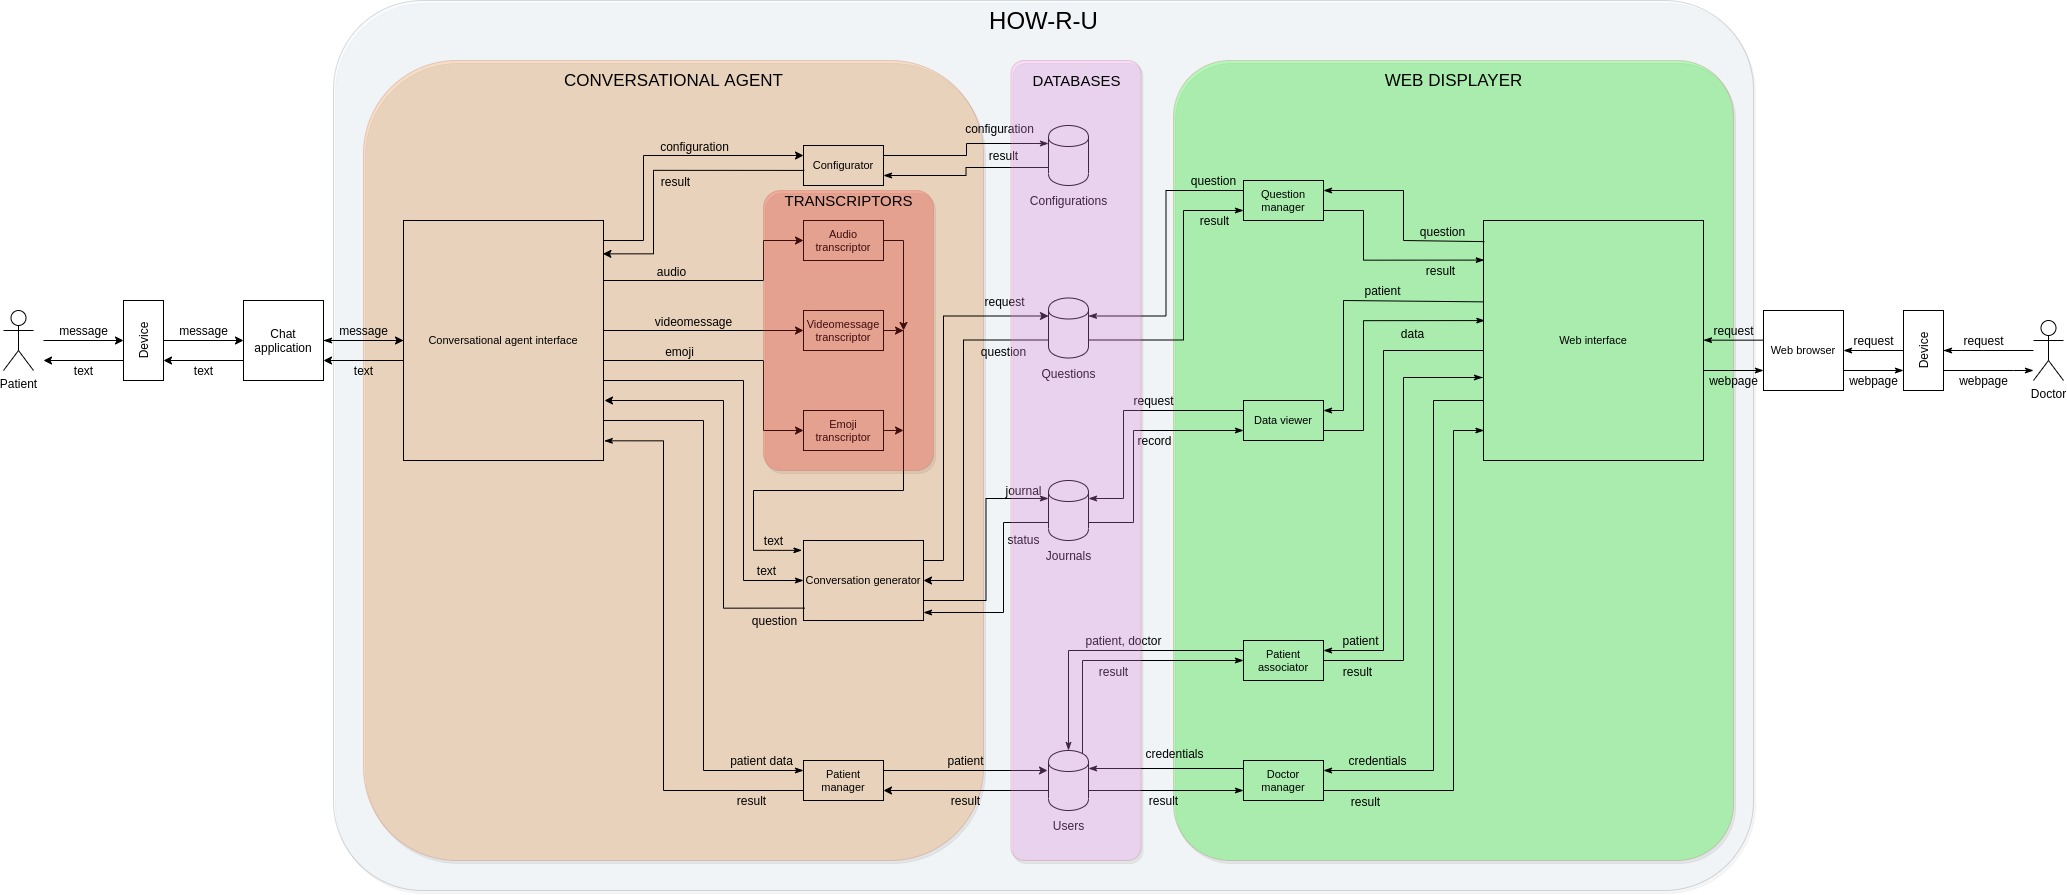
\includegraphics[width=\textwidth]{architecture.jpg}
  \caption{HOW-R-U architecture}
\end{figure}
\textcolor{red}{Explicar el diagrama (las cajas son módulos, los cuadrados componentes, discontinuos los opcionales, etc.)}



\subsection{Implementation}


\section{Evaluation}

\subsection{Experimental setup}

\subsection{Results}


\section{Discussion}

\section{Conclusions}

\newpage
\bibliographystyle{apacite}
\bibliography{refs}
\doclicenseThis

\end{document}
